\section{Method}
\label{sec:fullweak_method}

Training segmentation models using a combination of expensive pixel-wise annotations and other types of cheaper annotations, such as image-wise labels or single-pixel annotations is known to be beneficial, as well as using cross-task transfer learning techniques~\sidecite{Mensink}. This is motivated by empirical findings showing that, under a limited annotation budget, allocating a proportion of the budget to inexpensive image-level class labels led to superior performance compared to allocating the budget entirely to segmentation labels~\sidecite{Bearman16}. However, the optimal proportion of the budget to allocate per annotation type is a-priori unknown beforehand and data-dependent. Thus, the goal of our method is to find this data-specific optimal budget allocation in an online manner, as it is necessary for any dataset builder starting off.

We describe our method in the subsequent sections. For clarity, we focus on image segmentation and assume two kinds of annotations are possible: strong annotations as segmentation labels and weak annotations as image-level classification labels. Generalizing this formulation to other tasks or settings with more than two annotations types should follow directly.

\subsection{Problem formulation} 
Let $p_\textrm{data}(\x)$ be the distribution of training images for which we have no annotations initially. Each training image~$\x$ can be annotated with a pixel-wise segmentation labeling~{$(\x,\y)\sim{}p_\textrm{data}(\x)p_\textrm{sgm}(\y\mid\x)$} or an image-wise classification annotation~{$(\x,c)\sim{}p_\textrm{data}(\x)p_\textrm{cls}(c\mid\x)$}\sidenote{Without loss of generality, we assume that image-wise labels are a discrete class label, but that other kinds of annotations are equally valid as long as they are informative in the cross-task learning process.}. 
Sampling from the distributions $p_\textrm{cls}$ and~$p_\textrm{sgm}$ represents the task of manually annotating the image and has associated costs of~$\alpha_\textrm{c}>0$ and ~$\alpha_\textrm{s}>0$, respectively. Supported by previous work~\sidecite{Bearman16,Mensink,mahmood2022}, we will assume that $\alpha_\textrm{s}\gg\alpha_\textrm{c}$.

By sampling $C$~classifications from $p_\textrm{cls}$ and $S$~segmentation from ~$p_\textrm{sgm}$, we can build an annotated training dataset $\T=(\T_c,\T_s)\sim{}(p_\textrm{cls}^C, p_\textrm{sgm}^S)$. The dataset~$\T$ then has an annotation cost,
\begin{equation}
    \alpha_\textrm{c}C+\alpha_\textrm{s}S,
\end{equation}
which we assume to be bounded by an upper limit, or \emph{budget},~$B$.

To annotate $\T$, however, we can choose different \emph{allocation strategies}, or combinations of $C$ and~$S$, that have different costs and that yield different segmentation model performances. The utility~$u$ of an allocation strategy~$(C, S)$ is the expected performance of a model trained with datasets that follow that strategy,
\begin{equation}
    \label{eq:utility}
    u(C, S) = \mathbb{E}_{(\T_c,\T_s) \sim{}(p_\textrm{cls}^C, p_\textrm{sgm}^S)} \left[m(\T_c, \T_s)\right],
\end{equation}
\noindent
where~$m(\T_c, \T_s)$ is the performance score (\eg,~Dice score, IoU) of a segmentation model trained with datasets~($\T_c, \T_s$) and evaluated on a separate fixed test dataset. Note that in contrast to Active Learning, the utility is defined over the set of strategies~$(C,S)$ and not over the individual samples of a fixed training set. This is motivated by our aim to estimate the performance of the annotation strategy~$(C, S)$ and not the ensuing specific training dataset. 

%\begin{figure*}[h]
%\centering
%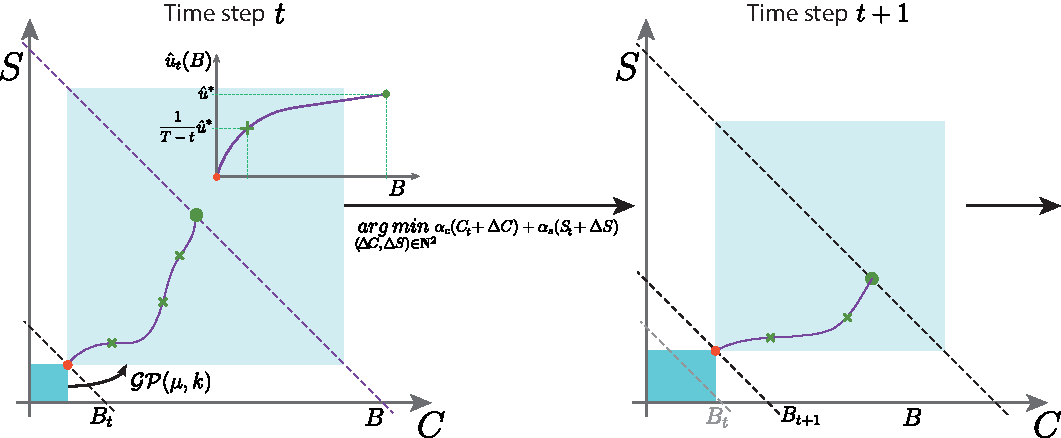
\includegraphics[width=\textwidth]{Figures/method.pdf}
%\caption{Illustration of proposed method. At a given iteration $t$, $C_t$ and $S_t$ classification and segmentation annotations have already been collected (blue region, left panel) with a budget of $B_t$. For the next annotation phase, the budget is increased to $B_{t+1}$. To determine how many new classification and segmentation annotations to collect, $M$ combinations of different quantities $(C^{(i)}, S^{(i)})$ are gathered according to Alg.~\ref{alg:build_gp_samples} to compute $m(C^{(i)}, S^{(i)})$. A Gaussian Process is then trained to estimate the utility of different combinations of annotation types (light blue area, left panel). From this, we infer $\Delta C$ and $\Delta S$ to select next by computing the combination that maximizes the expected improvement along the Pareto front given by the budget $B_2$ (red point, left panel). The next iteration starts then with the new proportions (red point, right panel) and follows the same steps (see text and Alg.~\ref{alg:the_algorithm} for details). For illustration purposes, the costs are set here to $\alpha_c=\alpha_s=1$.
%}
%\label{fig:method}
%\end{figure*}

\plainwidefig{1}{Figures/method.pdf}{Illustration of proposed method. At a given iteration $t$, $C_t$ and $S_t$ classification and segmentation annotations have already been collected (blue region, left panel) with a budget of $B_t$. For the next annotation phase, the budget is increased to $B_{t+1}$. To determine how many new classification and segmentation annotations to collect, $M$ combinations of different quantities $(C^{(i)}, S^{(i)})$ are gathered according to Alg.~\ref{alg:build_gp_samples} to compute $m(C^{(i)}, S^{(i)})$. A Gaussian Process is then trained to estimate the utility of different combinations of annotation types (light blue area, left panel). From this, we infer $\Delta C$ and $\Delta S$ to select next by computing the combination that maximizes the expected improvement along the Pareto front given by the budget $B_2$ (red point, left panel). The next iteration starts then with the new proportions (red point, right panel) and follows the same steps (see text and Alg.~\ref{alg:the_algorithm} for details). For illustration purposes, the costs are set here to $\alpha_c=\alpha_s=1$.}{fig:method}

Our goal then is to find the annotation strategy that maximizes the expected performance constrained to a budget~$B$,
\begin{equation}
\label{eq:the_optimization}
\begin{aligned}
    \max_{(C,S)\in\mathbb{N}^2} \quad & u(C, S), \\
    \textrm{s.t.} \quad & \alpha_cC+\alpha_sS \le B.
\end{aligned}
\end{equation}
In the following, we describe how we optimize Eq.~\eqref{eq:the_optimization}.

\subsection{Utility model}

As defined in Eq.~\eqref{eq:utility}, the utility function,~$u$, marginalizes over all possible training sets, which is intractable to compute in practice. To overcome this computational challenge, we approximate~$u$ with a collection~$\M$ of discrete samples, where each sample $m\in\M$ is a tuple containing an allocation strategy~$(C, S)$ and the estimated score $m(\T_c, \T_s)$ obtained for a dataset sampled with that allocation strategy. To build~$\M$, one could simply sample a random strategy~$(C', S')$, annotate a dataset~$(\T'_c, \T'_s)\sim{}(p_\textrm{cls}^{C'}, p_\textrm{sgm}^{S'})$, and measure its performance. However, this would imply annotating for different potential budgets and is thus infeasible in practice. Instead, a practical alternative is to leverage previously annotated data~$(\T_c, \T_s)$. For each sampled strategy~$(C', S')$, we build the corresponding dataset~$(\T'_c, \T'_s)$ by taking random samples from the already annotated data according to the strategy. While this procedure, formalized in Alg.~\ref{alg:build_gp_samples}, leads to biased samples, we empirically found this bias to have a minor impact on the final strategies compared to estimations with unbiased sampling.

\begin{algorithm}[t!] 
\caption{Build utility samples from annotated data}
\label{alg:build_gp_samples}
\begin{algorithmic}[1]
    \Function{BuildUtilitySamples}{$\T_c,\T_s$}
    \State $C \leftarrow |\T_c|$, $S \leftarrow |\T_s|$
    \State $\mathcal{M} \leftarrow \{((C, S), m(\T_c,\T_s))\}$ \Comment{Add sample with all the available data}
    \Repeat {$M-1$}
    \State Sample $(C', S')\in[0, C]\times[0, S]$
    \State $\T'_c \leftarrow$ \{$C'$~elements sampled from $\T_c$\}
    \State $\T'_s \leftarrow$ \{$S'$~elements sampled from $\T_s$\}
    \State $\mathcal{M} \leftarrow \mathcal{M} \cup ((C', S'), m(\T'_c, \T'_s))$ 
    \EndRepeat
%    \State \Return $\mathcal{M}$
    \EndFunction
\end{algorithmic}
\end{algorithm}

While $\M$~provides an estimation of~$u$ as a set of discrete locations, we generalize these estimations to the entire space of strategies by fitting a Gaussian Process~(GP) to the samples in~$\M$. The Gaussian Process, $\mathcal{GP}(\mu, k)$ is parameterized by a suitable mean function~$\mu$ and covariance function~$k$. 

In our case, we use the mean function,
\begin{equation}
    \mu(C, S) = \gamma_c\log(\beta_cC+1) + \gamma_s\log(\beta_sS+1),
    \label{eq:gp_mean}
\end{equation}
which accounts for the fact that the segmentation performance increases logarithmically with the volume of the training data~\sidecite{sun2017} and that each annotation type has a different rate of performance growth. Similarly, the covariance~$k$ is a combination of two RBF~kernels with different scales~$\ell_c$, $\ell_s$ for each annotation type,
\begin{equation}
    k\left((C, S), (C', S')\right) = \sigma^2\exp\left(-\frac{(C-C')^2}{2\ell_c^2}\right) \exp\left(-\frac{(S-S')^2}{2\ell_s^2}\right).
\end{equation}
The values~$\gamma_c$, $\beta_c$, $\gamma_s$, $\beta_s$ from the mean, the length scales~$\ell_c$, $\ell_s$ and the amplitude~$\sigma$ from the covariance are trainable parameters of the~GP.


The trained GP models a distribution over utility functions, $u \sim\mathcal{GP}(\mu, k)$, that are plausible under the samples~$\M$. This distribution represents not only the expected utility, but also its uncertainty in different areas of the strategy space. Sampling just a single~$u$ from the GP to solve Eq.~\eqref{eq:the_optimization} would thus be suboptimal. For this reason, we substitute the utility~$u$ in Eq.~\eqref{eq:the_optimization} by a surrogate function~$\hat{u}$ that trades-off exploitation and exploration, thus incorporating uncertainty information into the optimization problem. Following a Bayesian optimization approach~\sidecite{jones1998efficient}, we choose~$\hat{u}$ to be the expected improvement~(EI),
\begin{equation}
    \hat{u}(C, S) = \mathbb{E}_{u\sim\mathcal{GP}_t}[\max\{u(C, S) - m^*, 0\}],
    \label{eq:EI}
\end{equation}
where~$m^*$ is the current maximum point.

\subsection{Optimization}

Training the GP requires annotated data to build the set~$\M$, which in turn relies on an annotation strategy that we are trying to find, whereby implying a circular dependency. We address this circular dependency by optimizing Eq.~\eqref{eq:the_optimization} in an iterative manner.

\cref{alg:the_algorithm} allocates the available budget~$B$ in a fixed number of adaptive installments, alternating between data annotation with the current strategy, GP~fitting, and strategy selection for the next budget installment. More specifically, our method starts with an initial strategy~$(C_0, S_0)$ with associated cost~$B_0$. At each iteration~$t$, new data is annotated according to the current strategy~$(C_t, S_t)$ so that the sets of annotated data~$(\T_c, \T_s)$ contain $C_t$~classification and $S_t$~segmentation annotations, respectively. From the available annotated data~$(\T_c, \T_s)$, we extract new samples for~$\M$ and fit the GP, which defines the surrogate function~$\hat{u}_t$. The corresponding current maximal point~$m^*_t$ is set to be the maximum performance found so far\sidenote{We assume that this corresponds to the performance of the model trained with all the annotated data available at this iteration.}, $m^*_t=m(\T_c, \T_s)$. Finally, this surrogate function is used to estimate the next best strategy~$(C_{t+1}, S_{t+1})$. We find a delta strategy~$(\Delta{}C,\Delta{}S)$ that increases the expected improvement by a fixed fraction of its maximum possible value,
\begin{equation}
\begin{aligned}
    \argmin_{(\Delta{}C,\Delta{}S)\in\mathbb{N}^2} \quad & \alpha_c (C_t + \Delta{}C)+\alpha_s (S_t + \Delta{}S), \\
    \textrm{s.t.} \quad & \hat{u}_t(C_t + \Delta{}C, S_t + \Delta{}S) \ge \dfrac{1}{T - t}\hat{u}^*_t,
\end{aligned}
\label{eq:delta_strategy}
\end{equation}
where $T$~is the desired maximum number of iterations of the algorithm and~$\hat{u}_t^*$ is the maximum expected improvement that can be reached using the entire budget~$B$ for the current surrogate function~$\hat{u}_t$ according to Eq.~\eqref{eq:the_optimization}. The found delta strategy defines the new strategy~$(C_{t+1}, S_{t+1}) = (C_t + \Delta{}C, S_t + \Delta{}S)$ for the next iteration. The process is depicted in~\cref{fig:method}.

\begin{algorithm}[]
\caption{Proposed approach}
\label{alg:the_algorithm}
\begin{algorithmic}[1]
\Require Number of iterations~$T$, initial labelling strategy~$(C_0, S_0)$
\State $t\leftarrow 0$, $\Delta{}C\leftarrow C_0$, $\Delta{}S\leftarrow S_0$, $\T_c=\emptyset$, $\T_s=\emptyset$, $\mathcal{M}=\emptyset$
\While {$t<T$}
\State Annotate new data $(\Delta{}\T_c,\Delta{}\T_s)\sim{}(p_\textrm{cls}^{\Delta{}C}, p_\textrm{sgm}^{\Delta{}S})$
\State $\T_c \leftarrow \T_c \cup \Delta{}\T_c, \quad \T_s \leftarrow \T_s \cup \Delta{}\T_s$ \Comment{Note that $|\T_c|=C_t$ and $|\T_s|=S_t$}
\State $\mathcal{M} \leftarrow \mathcal{M} \,\cup\,$\Call{BuildUtilitySamples}{$\T_c$, $\T_s$} % \Comment{See Alg.~\ref{alg:build_gp_samples}}
\State Train GP with samples in~$\mathcal{M}$
\State Compute $(\Delta{}C, \Delta{}S)$ from Eq.~\eqref{eq:delta_strategy}
\State $C_{t+1} \leftarrow C_t + \Delta{}C, \quad S_{t+1} \leftarrow S_t + \Delta{}S$
\State $t\leftarrow t+1$
\EndWhile
\Ensure $(C_T, S_T)$
\end{algorithmic}
\end{algorithm}

Note that solving Eq.~\eqref{eq:delta_strategy} requires finding~$\hat{u}_t^*$, which in turn requires solving Eq.~\eqref{eq:the_optimization}. While solving two optimization problems may seem unnecessary, the solutions of both problems are in the Pareto front\sidedef{Pareto front}{Set of non-dominated strategies for which no other strategy has simultaneously smaller cost and larger or equal expected improvement} of strategies. Given that the space of strategies is discrete, the elements of the Pareto front can be easily found in linear time by enumerating all possible strategies, computing their costs and expected improvements with~$\hat{u}_t$, and discarding the dominated elements. Given the Pareto front, the strategy with the maximum EI~$u^*_t$ and the strategy of minimum budget with EI larger than $\frac{1}{T - t}\hat{u}^*_t$\sidenote{Solutions of Eq.\eqref{eq:the_optimization} and Eq.~\eqref{eq:delta_strategy}, respectively.}, can be found in linear time.

\iffalse
\subsection{Iterative approximation}
To overcome the second challenge of solving Eq.~\eqref{eq:the_optimization}, we chose to optimize the function sequentially by allocating the available budget~$B$ in small installments of size~$\Delta{}B$. 

In Alg.~\ref{alg:the_algorithm}, we summarize our iterative approach where at each iteration~$t$, new data is labelled according to the current strategy~$(C_t, S_t)$ so that the sets of annotated data~$(\T_c, \T_s)$ contain $C_t$~classification and $S_t$~segmentation annotations, respectively. 
\begin{algorithm}[!b]
\caption{Proposed approach}
\label{alg:the_algorithm}
\begin{algorithmic}[1]
\Require Number of iterations~$T$, budget step~$\Delta{}B$, initial labelling strategy~$(C_0, S_0)$
\State $t\leftarrow 0$, $\Delta{}C\leftarrow C_0$, $\Delta{}S\leftarrow S_0$, $\T_c=\emptyset$, $\T_s=\emptyset$, $\mathcal{M}=\emptyset$
\While {$t<T$}
\State Annotate new data $(\Delta{}\T_c,\Delta{}\T_s)\sim{}(p_\textrm{cls}^{\Delta{}C}, p_\textrm{sgm}^{\Delta{}S})$
\State $\T_c \leftarrow \T_c \cup \Delta{}\T_c, \quad \T_s \leftarrow \T_s \cup \Delta{}\T_s$ \Comment{Note that $|\T_c|=C_t$ and $|\T_s|=S_t$}
\State $\mathcal{M} \leftarrow \mathcal{M} \,\cup\,$\Call{BuildGPSamples}{$\T_c$, $\T_s$} \Comment{See Alg.~\ref{alg:build_gp_samples}}
\State Train GP with samples in~$\mathcal{M}$
\State Compute $(\Delta{}C, \Delta{}S)$ from Eq.~\eqref{eq:optimization_step}
\State $C_{t+1} \leftarrow C_t + \Delta{}C, \quad S_{t+1} \leftarrow S_t + \Delta{}S$
\State $t\leftarrow t+1$
\EndWhile
\Ensure $(C_T, S_T)$
\end{algorithmic}
\end{algorithm}
The available annotated data~$(\T_c, \T_s)$ is then used to build~$M$ new samples for~$\mathcal{M}$ following the method described in Alg.~\ref{alg:build_gp_samples}. This sampling prioritizes elements close to the current strategy~$(C_t, S_t)$ to build more accurate approximations of~$u$ in the region where the next strategy will be found and also to account for the fact that the space of strategies below~$(C_{t-1}, S_{t-1})$ has already been sampled during the previous iterations (see Fig.~\ref{fig:method}). While the elements of~$\mathcal{M}$ should ideally be sampled from the original data and annotation distributions, this would involve additional costs. Instead, we sample them from the sets of already annotated data. While this biases the estimation of the~GP, we empirically found this bias to have a minor impact on the final strategies compared to estimations with unbiased sampling.

Once the set of samples~$\mathcal{M}$ has been updated, we train a GP using these. %leading to accurate estimations of the utility function around the current strategy~$(C_t, S_t)$.
We can then use this GP to find the optimal delta strategy~$(\Delta{}C, \Delta{}S)$ for a budget increase of $\Delta{}B$ by solving,
\begin{equation}
\label{eq:optimization_step}
\begin{aligned}
    \max_{(\Delta{}C,\Delta{}S)\in\mathbb{N}^2} \quad & \hat{u}_t(C_t + \Delta{}C, S_t + \Delta{}S), \\
    % \textrm{s.t.} \quad & (C_t + \Delta{}C)\alpha_c + (S_t + \Delta{}S)\alpha_s \le \Delta{}B\cdot{}t,
    \textrm{s.t.} \quad & \alpha_c\Delta{}C + \alpha_s\Delta{}S \le \Delta{}B.
\end{aligned}
\end{equation}
where~$\hat{u}_t$~is a surrogate function for~$u$ obtained from the~GP. Following a Bayesian optimization approach~\sidecite{jones1998efficient}, we model~$\hat{u}_t$ as the expected improvement~(EI),
\begin{equation}
    \hat{u}_t(C, S) = \mathbb{E}_{u\sim\mathcal{GP}_t}[\max\{u(C, S) - m^*_t, 0\}],
    \label{eq:EI}
\end{equation}
where~$m^*_t=m(\T_c, \T_s)$ is the best performance found so far, \ie,~the performance of the model trained with all the available annotated data.


\begin{algorithm}[t!]
\caption{Build GP samples from labelled data}
\label{alg:build_gp_samples}
\begin{algorithmic}[1]
    \Function{BuildGPSamples}{$\T_c,\T_s$}
    \State $C \leftarrow |\T_c|$, $S \leftarrow |\T_s|$
    \State $\mathcal{M} \leftarrow \{((C, S), m(\T_c,\T_s))\}$ \Comment{Add element with all the available data}
    \Repeat {$M-1$}
    \State Sample $(C', S')\in[0, C]\times[0, S]$ with probability proportional to~$\|(C',S')\|_2$
    \State $\T'_c \leftarrow$ \{$C'$~elements sampled uniformly from $\T_c$\}
    \State $\T'_s \leftarrow$ \{$S'$~elements sampled uniformly from $\T_s$\}
    \State $\mathcal{M} \leftarrow \mathcal{M} \cup ((C', S'), m(\T'_c, \T'_s))$ 
    \EndRepeat
    \State \Return $\mathcal{M}$
    \EndFunction
\end{algorithmic}
\end{algorithm}

Assuming that the utility is monotonically increasing with respect to $C$ and~$S$, the solution to Eq.~\eqref{eq:optimization_step} is in the Pareto front of strategies for which no other strategy with cost lower than~$\Delta{}B$ has simultaneously more class-labelled and more segmentation-labelled elements (\ie, the set of non-dominated feasible strategies). Note that the size of the Pareto front grows linearly with~$\Delta{}B$ and its elements can be easily enumerated. Hence, Eq.~\eqref{eq:optimization_step} can be efficiently solved by enumerating the strategies of the Pareto front and keeping the strategy with highest~EI (see Fig.~\ref{fig:method}).
\fi